\section{Selection Variables \label{sec:SelVar}}
HSCPs can be distinguished from SM particles in CMS due to their high momentum and slow speed.
The momentum of a particle can be determined by its bending in the magnetic field of CMS.
The slow speed of HSCPs lead to two interesting detector signatures. The first is that the particles will arrive at the detector elements later than SM particles will.
The muon system, being the furthest detector element from the interaction point, has the largest timing difference. The measurement of the arrival time of particles in the
muon system is discussed in Ch.~\ref{sec:timing}. The \invbeta\ variable is used in the searches to discriminate between HSCPs and SM particles.
The second interesting signature is that HSCPs have a larger amount of ionization energy loss per unit length 
than SM particles of the same momentum, as discussed below.

\subsection{Transverse Momentum Measurement \label{sec:PMeasurement}}
A muon passing through CMS will likely be reconstructed three times~\cite{2012JInst...7P0002T}; once only in the silicon tracker, referred to as a tracker track;
once only in the muon system, referred to as a stand-alone muon; and once as a combined track found in both the muon system and silicon tracker, referred
to as a global muon. CMS measures the curvature of a track which is proportional to, and can be used to determine, the $Q/p_T$ of the track.
In the central region of CMS, tracker tracks have a resolution on $Q/p_T$ of 1\% for muons at intermediate momentum and 7\% at
high momentum with the resolution being approximately
twice as large in the forward region. Intermediate momentum is defined as 15--100~GeV/$c$ and high momentum is defined as 400--1000 GeV/$c$.
Stand-alone muons in the central region have a resolution on $Q/p_T$ of 8\% for intermediate momentum and 25\%~\cite{2008AN097} for high momentum with the uncertainty again
being about twice as large in the forward region. The resolution for global muons is the same as for tracker muons for intermediate momentum and is slightly better
than tracker muons at high momentum at 6\% in the central region.

The \muononly\ analysis uses the $p_T$ measurement coming from the stand-alone muon while the rest of the analyses use the measurement from the tracker track.
The tracker track momentum is used even when the global muon is available due to issues specific to $R$-hadrons.
$R$-hadrons are unlikely to undergo a nuclear interaction while traversing the silicon tracker so they would have the same electric charge at all points in the tracker.
However, $R$-hadrons will often undergo a nuclear interaction with other parts of CMS while they pass through the detector. 
The parts of CMS
where this is most likely to happen are the calorimeter, magnet coil  and cryostat, and the steel return yoke in the muon system.
This makes their tracks curve differently inside of CMS than muons and has the possibility for the $R$-hadron's momentum to be misreconstructed.

The \pt\ measurement by the stand-alone muon is especially sensitive to the $R$-hadron interacting with the steel return yoke.
Interacting with the steel return yoke allows for the electric charge of $R$-hadrons to change in the middle of the muon system.
This means that the average value of $Q$ during their passage through the muon system may not equal $1e$.
This affects the momentum measurement as a charge of $Q=1e$ is assumed when converting the measured $Q/p_T$ to $p_T$.
This effect has different consequences for the stop and gluino samples.

A stop particle, specifically not an anti-stop, has a charge of $+(2/3)e$ and forms an $R$-hadron with either an anti-quark ($\tilde{t} \bar{q}$) or
two quarks  ($\tilde{t} q q$). Anti-quarks have a charge of $-(2/3)e$ or $+(1/3)e$ leading to $R$-hadrons with a charge
of either 0 or $+1e$. Quarks have a charge of either $+(2/3)e$ or $-(1/3)e$ which allows for
the creation of $R$-hadrons with a charge of 0, $+1e$, or $+2e$. Thus a stop $R$-hadron will always have a
positive charge or be neutral. For an anti-stop, the effect is reversed and the $R$-hadron will always have a
negative charge or be neutral.

For gluino $R$-hadrons this statement does not hold true. Gluinos can hadronize into glue balls ($\tilde{g}g$), $R$-mesons ($\tilde{g} q \bar{q}$), or
$R$-baryons  with either quarks or anti-quarks ($\tilde{g} qqq$ or $\tilde{g} \bar{q}\bar{q}\bar{q}$),
allowing the charge of the $R$-hadron to range from $-2e$ to $+2e$. This leads to the
average charge of the $R$-hadron as it traverses the muon system to often be less than $1e$ and the $p_T$ value to be overestimated allowing for further separation
between HSCP and SM particles.

To observe this effect the unitless function
$\Delta(Q/p_T)$ is defined in Equation~\ref{eq:deltaqopt}
\begin{equation}
\Delta(Q/p_T) = \frac{((Q/p_T)_{SA} - (Q/p_T)_{Tk})}{(Q/p_T)_{Tk}}
\label{eq:deltaqopt}
\end{equation}
where ``SA'' refers to stand-alone muon qualities and ``Tk'' refers to
tracker track qualities. As the $p_T$ resolution of tracker tracks is much better than for stand-alone muons, it is a sufficiently good approximation
of the true particle momentum. Figure~\ref{fig:MuOnlyInvPtDiff} shows the distribution of
$\Delta(Q/p_T)$ for tracks with inner track $p_T > 200$ GeV/$c$
for data and various simulated HSCP signal samples.
A value of zero in this plot indicates the $p_T$ was reconstructed correctly
while negative one indicates the reconstructed $p_T$ approaches infinity.
The CD stau sample, which does not change charge,
has a distribution similar to data, though slightly wider.
The slight discontinuity at negative one is due to particularities of the reconstruction but only affects a small number of tracks.
The stop sample, which is not able to flip charge but merely to switch
between one sign and zero, is centered at zero but with a slightly wider
width than data or CD stau.
The gluino sample, which can flip charge, is centered closer to negative one.
This means that
the reconstructed $p_T$ is normally larger than what is generated, sometimes
to a very large degree. This increases the differences between gluino HSCPs and the background.

\begin{figure}
 \begin{center}
  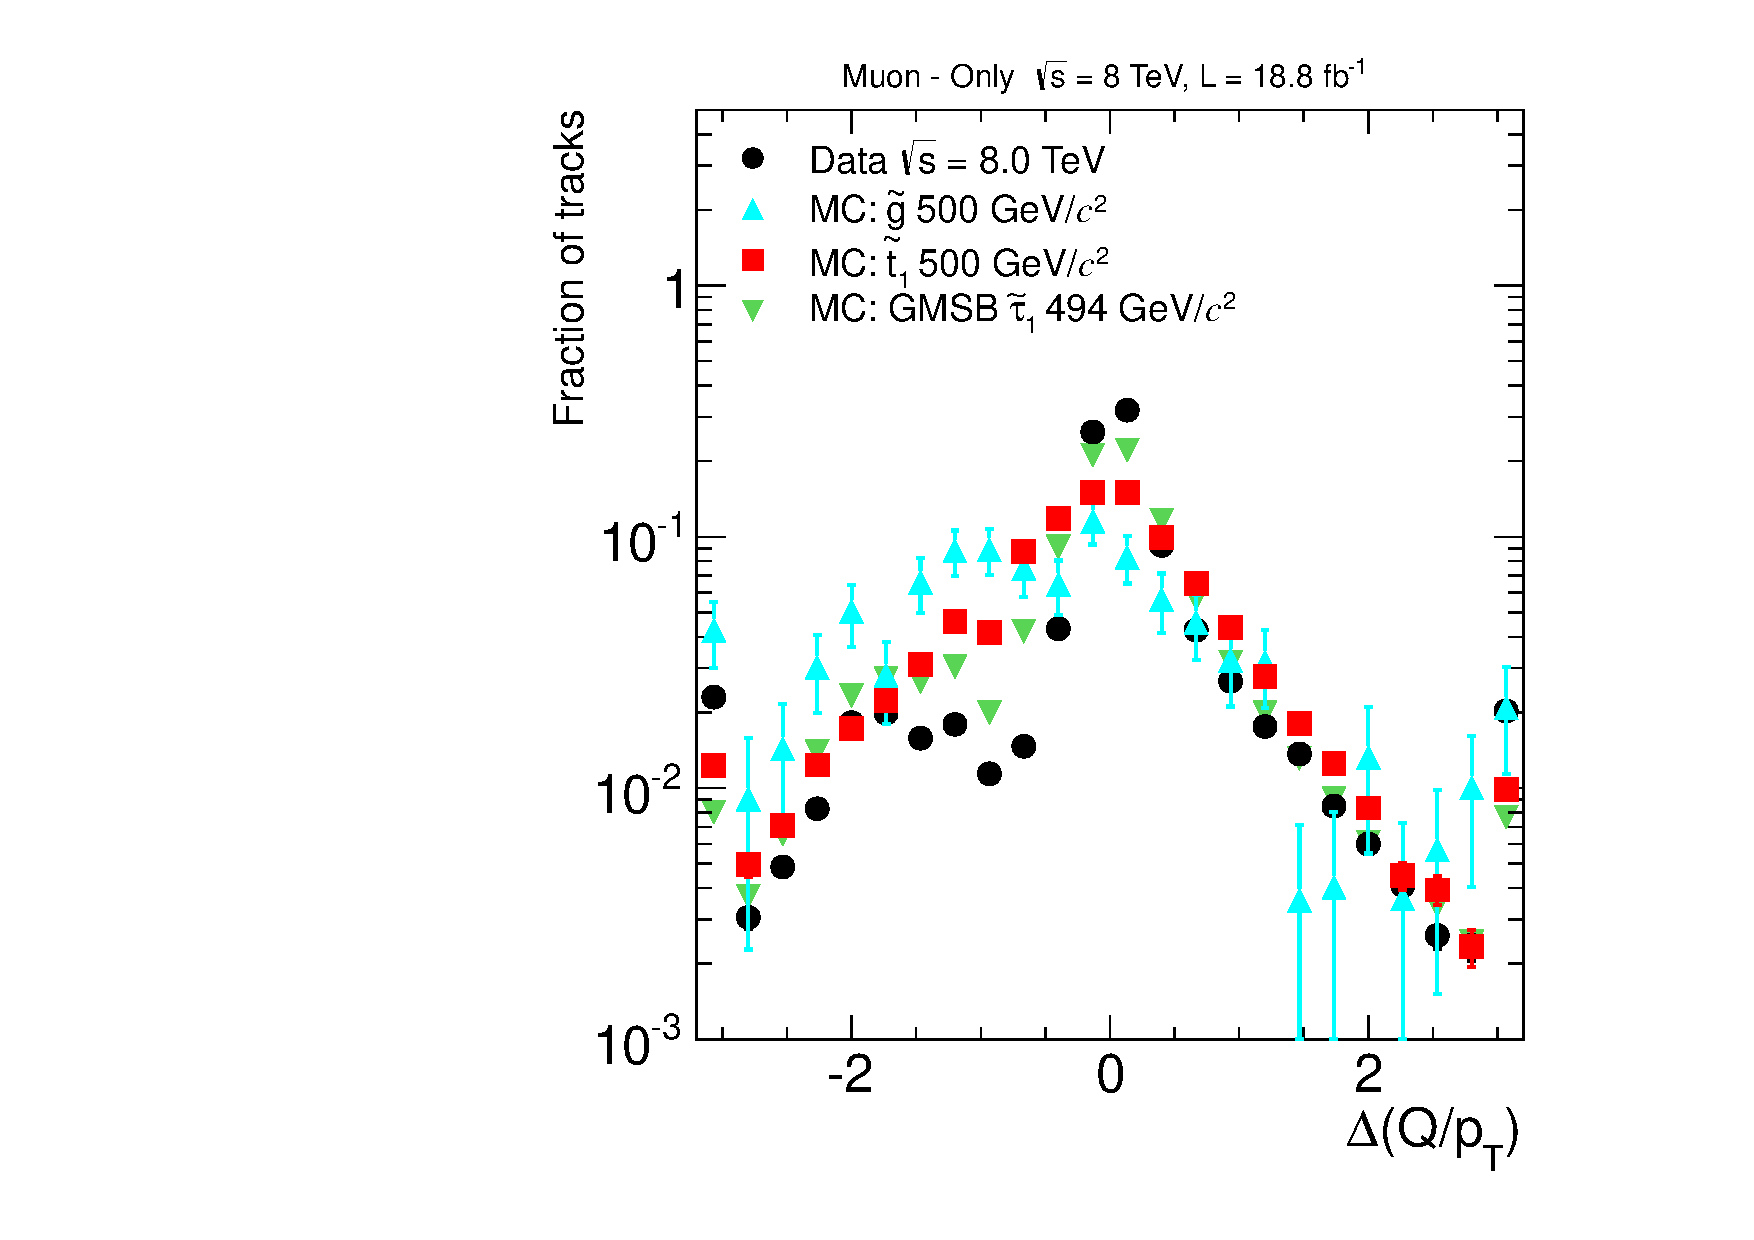
\includegraphics[width=0.7\textwidth]{figures/muonly/Selection_Comp_Signal_8TeV_InnerInvPtDiff_BS}
 \end{center}
 \caption{Distribution of $\Delta(Q/p_T)$
    for data, 500 GeV/$c^2$ gluino, 500 GeV/$c^2$ stop, and 494 GeV/$c^2$ CD stau. The $y$-axis is in log scale.
    \label{fig:MuOnlyInvPtDiff}}
\end{figure}

For the lepton like samples with non-unit charge, the \pt\ will be mismeasured by a factor of $1/Q$. This means that multiply 
charged particles will have their \pt\ underestimated making them somewhat harder to separate from backgrounds.
This effect can be seen in Figure~\ref{fig:RecoGenPt}.
%For the lepton like samples with non-unit charge the \pt\ will be mismeasured by a factor of 1/Q, meaning fractionally charged particles will have their \pt\ overestimated
%while multiply charged particles will be underestimated. This effect can be seen in Figure~\ref{fig:RecoGenPt}.

\begin{figure}
 \begin{center}
  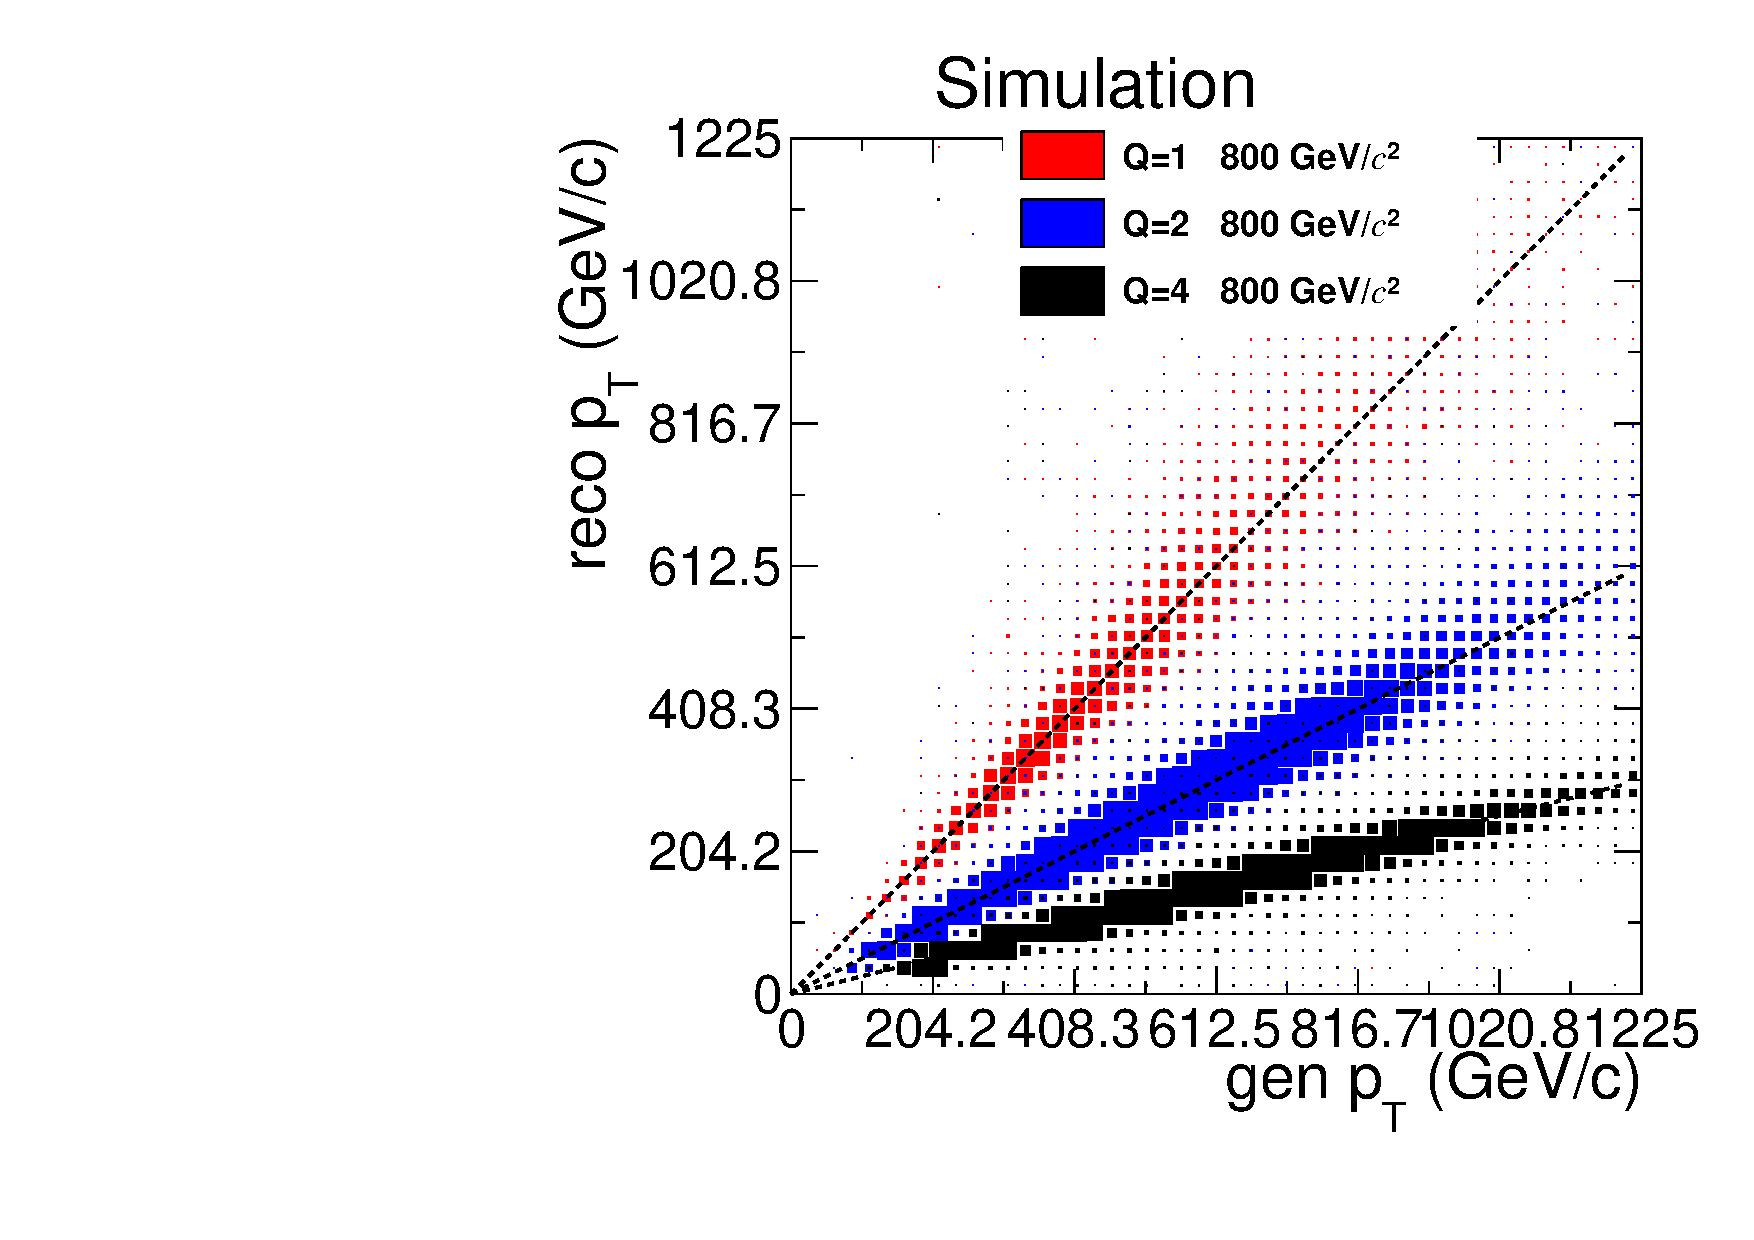
\includegraphics[width=0.44\textwidth]{figures/tkonly/SIM_Validation_Pt.pdf}
 \end{center}
 \caption{Distribution of reconstructed $p_T$ versus generator $p_T$ for Q=1e, 2e, and 4e samples.
    \label{fig:RecoGenPt}}
\end{figure}

\subsection{Energy Loss Measurement \label{sec:DedxMeasurement}}
The amount of ionization energy a particle loses while traversing CMS can be measured by the silicon tracker.
%that a slow moving HSCP will have a larger ionization energy loss in the silicon tracker than SM particles will.
For particles with 0.1 $\lesssim \beta \gamma \lesssim$ 1000, where $\gamma$ is $1/\sqrt{1 - \beta^2}$,
the average amount of the ionization energy loss per unit length in a given material, \dedx, is to a large degree dependent only on the velocity of the particle
and its charge as described by the Bethe-Bloch formula~\cite{PDG}.
The dependence of \dedx\  on charge varies approximately as $Q^2$, meaning that even a $Q=2e$ HSCP will have almost four times as much energy loss as a SM particle. 
The dependence on speed for particles with $0.1 < \beta < 0.9$ varies approximately as $1/\beta^2$; so slow moving HSCP would have large \dedx\ values.
At higher speeds, the energy loss has a broad minimum up to $\beta \gamma$ of 1000.
Particles in this broad minimum all have close to the same energy loss and are generically referred to as minimum ionizing particles (MIP).
Above this level, radiative effects become important as they cause very rare, very high-energy losses that result in an increase to the average energy loss.
Techniques described below are used to help mitigate the effect of this radiative rise.
%Experimental techniques are used to reduce the impact of these rare high-energy losses so that
%SM particles with a momentum above 10~GeV will all have mean \dedx\ close to the minimum value
%($\approx$ 3MeV/cm) and are referred to as minimum ionizing particles (MIPs).

A short description of the \dedx\ measurement is included here, a more detailed description can be found in~\cite{2010EPJC...70.1165K, Khachatryan:2011ts, Quertenmont:1361029}.
As in~\cite{Chatrchyan:2012sp}, two variables related to \dedx\ are calculated for each track. 
The first, \ih, is an estimator of the average \dedx\ of the track. It can be used in combination with the momentum measurement to estimate the mass of a particle.
The second, \ias, is a discriminant that is designed to give the best separation between MIPs and high-ionizing particles.
The same measurements are used to determine \ih\ and \ias\ so the variables are not independent.

\ih\ is calcualted as the harmonic mean of the \dedx\ measurements along the track;
\begin{equation}
 I_h= \biggl( \cfrac{1}{N} \sum_i c_{i}^{-2} \biggr)^{-1/2},
 \label{eq:HarmonicEstimator}
\end{equation}
where $N$ is the number of measurements in the silicon-strip tracker and $c_{i}$ is the energy loss per unit path length
of the $i$th measurement. The use of a harmonic mean greatly reduces the impact of the rare radiative losses as the highest energy
losses are effectively given less weight than lower energy losses. This leads to all
SM particles produced at the LHC with momentum above 10~GeV/$c$ on average having \ih\ values close to the minimum value ($\approx$ 2.8~MeV/cm). 
HSCP will have high \ih\ as their energy loss is consistently large.

The second variable is \ias\ which is a modified version of the Smirnov-Cramer-von Mises~\cite{Eadie, James} discriminant.
The discriminant is given by:
\begin{equation}
 I_{as} = \frac{3}{N} \times \left(
   \frac{1}{12N} + \sum_{i=1}^N
   \left[
   P_i \times \left( P_i - \frac{2i-1}{2N} \right)^2 \right] \right),
\end{equation}
where $P_i$ is the probability for a MIP to
produce a charge smaller or equal to that of the $i$th measurement in the silicon-strip tracker
for the observed path length in the detector, and the sum is over the
measurements ordered in terms of increasing $P_i$. The probabilities are found from tracks with momentum greater than five~GeV/$c$ collected with a trigger requiring only
that a proton collision occured inside CMS.
The discriminant is peaked at zero for MIPs and approaches one for high-ionizing particles.

An estimate of the mass $m$, assuming Q=1$e$, of a particle can be made from \ih\ and the momentum $p$ of a track. This is done by using Eq.~\ref{eq:MassFromHarmonicEstimator};
\begin{equation}
I_h= K\cfrac{m^2}{p^2}+C.
\label{eq:MassFromHarmonicEstimator}
\end{equation}
with  $K=2.559 \pm 0.001$ MeV cm$^{-1}$ $c^2$ and $C=2.772 \pm 0.001$ MeV cm$^{-1}$ as determined from low momentum protons~\cite{Khachatryan:2011ts}.
Eq.~\ref{eq:MassFromHarmonicEstimator} is an approximation that works well over the range $0.1 < \beta < 0.9$~\cite{PDG}.